
\subsection{Sequential Algorithm}
For sequential algorithms, the generic algorithm is expanded to look something like this:

\begin{minted}{cpp}
Generic Sequential Convolution Algorithm

read input.wav into x
read filter.wav into h
/*Find peak of input*/
peakIn = 0
for i in x:
    if | i | > peakIn:
        peakIn = i
        
/*Convolve*/
y = convolve(x,h)

/*Find peak of output*/
peakOut = 0
for i in y:
    if | i | > peakOut:
        peakOut = i
/*Scale all points in output*/
for n in y:
    n = n * peakIn / peakOut

/*(Optional) Write to output file*/
write y to output.wav
\end{minted}
\subsubsection{Time Domain Convolution}
\indent \par As explained in the background section, the equation for full convolution is:
$$y[n] = \sum_{k=0}^{K-1} x[n-k] \cdot h[k]$$

A direct transliteration of the summation, where $Y = N + K -1$ or the length of the output, would look like this:

\begin{minted}{cpp}
Direct Transliteration of Convolution Equation

for n [0, Y):
    y[n] = 0
    for k [0, K):
        if (n - k < N):
            y[n] += x[n - k] * h[k]
\end{minted}
The problem is that this has a high probability of cache misses. Cache is temporary storage inbetween memory and the \gls{cpu}. When a program asks for a value in an array or somewhere in memory, an entire block of memory (typically 64 bytes or 8 floating point numbers) is stored in the cache. This takes some extra time, but it becomes useful if the program utilizes the rest of the numbers in the block. The retrieval of the data from memory to cache takes longer than retrieval of data from cache to \gls{cpu}. Therefore, programs that access memory sequentially are more likely to be retrieving from cache with fewer trips to the main memory and are therefore faster. The previous code snippet had \verb|x[n-k]| where \verb|n| and \verb|k| increase, \verb|k| faster than \verb|n|. Because of this, \verb|x| is being accessed in reverse then jumping forward in time.


\begin{minted}{cpp}
Optimized Convolution Algorithm

/*Set all values in y to zero first*/
for n in y:
    n = 0
    
for k [0, K):
    for n [0, N):
        y[k + n] += x[n] * h[k]
\end{minted}
Where K = length of h and N is the length of x.

\noindent This was lightly tested for K = 480,000 and N = 2,304,000. All trials were done on different \gls{cpu}s, but each trial was done on the same \gls{cpu}. 

\begin{center}
Speed Benchmarks for Cache-Unfriendly vs Cache-Friendly
\begin{tabular}{ c c c c c }
 Trial Number & Cache Unfriendly & Cache Friendly & Speedup amount & Percent speedup (floor)\\ 
 1 & 4,878.2635 s & 3,292.94750 s & 1,585.61600 s & 32 \\  
 2 & 4,987.8665 s & 3,801.66950 s & 1,186.19700 s & 23 \\
 3 & 5,214.8175 s & 3,707.61700 s & 1,507.20050 s & 28 \\
 4 & 4,713.9980 s & 3,228.36475 s & 1,485.63325 s & 31 \\
 5 & 4,887.9455 s & 3,417.36225 s & 1,470.58325 s & 30
\end{tabular}
\end{center}

In audio terms, this input is tiny. At 96 kHz, it's only 24 seconds long. Longer inputs will have more drastic differences and larger percentages.

Taking the cache into account, my full time domain convolution algorithm looks like this:

\begin{minted}{cpp}
Time Domain Convolution Algorithm

read input.wav into x
read filter.wav into h
/*Find peak of input*/
peakIn = 0
for i in x:
    if | i | > peakIn:
        peakIn = i
        
/*Convolve*/
for n in y:
    n = 0
for k [0, K):
    for n [0, N):
        y[k + n] += x[n] * h[k]
        
/*Find peak of output*/
peakOut = 0
for i in y:
    if | i | > peakOut:
        peakOut = i
/*Scale all points in output*/
for n in y:
    n = n * peakIn / peakOut

/*(Optional) Write to output file*/
write y to output.wav
\end{minted}

\subsubsection{Frequency Domain Convolution}

Also stated in the background section, the formula for frequency domain convolution is:

$$y = F^{-1}(F(x) \cdot F(h))$$
\paragraph{Padding Considerations} \hspace{0pt} \\
\indent While the Fourier transform is not covered in this paper, there are several important aspects of the Fourier transform and the convolution theorem that affect the padding of the signal.

A crucial aspect of the \gls{dft} is that each index of the transformed, discrete signal corresponds to a certain analysis frequency, and the value of that index is the energy of that frequency. The analysis frequency at each index is determined by the number of samples of the pre-transformed/transformed signal and the sample rate of the audio. The implication of this is that the filter's frequency bins must align with the input's frequency bins in order for the pointwise multiplication to make sense. So the filter must be padded with 0's so that it is of length N before taking the \gls{dft} of the signal. 

As stated earlier, the FFT is a specific implementation of the \gls{dft} that reduces the number of necessary computations. This operates by a divide and conquer algorithm that will operate faster the lower the least prime factor of the input is. Meaning, the FFT is the fastest when the signal is a power of 2. To make the FFT perform faster, the two signals must be padded with zeroes to the next largest factor of 2. The padded length = $2^{\ceil{\log_2N}}$.

Lastly, the convolution theoreum states that pointwise multiplication in the frequency domain is convolution in the time domain but more specifically \textit{circular} convolution. Circular convolution is different from full convolution in how it changes the assumption about out of bounds values. The assumption for full convolution was that all out of bounds values of x are 0. Circular convolution makes the assumption that negative indices of x will refer to the end of x. $x[-K + 1:-1] = x[N - K: N - 1]$ Because data at the end of a signal doesn't usually relate to the beginning of a signal, we pad the input with at least K - 1 zeross to prevent the circularity and force those out of bounds values to become 0. 

\vspace{5mm}
After all of these considerations, the size of the padded FFT input($P$) should be $P = 2^{\ceil{\log_2(Y)}}$, where $Y = N + K - 1$.

\paragraph{FFTW3} \hspace{0pt} \\
\indent FFTW3 is the name of the Fourier transform library that I used. It provides memory allocation wrappers for complex inputs and real inputs to ensure that they are optimized for speed. Then, in order to execute a Fourier Transform, a plan needs to be created with the parameters for the transform. There are also specific \glspl{api} meant for the transform of one dimensional, real valued inputs. The library typically uses double precision floating point values. I'm choosing to use single precision floating point variant by putting "f" on the end of every \gls{api}. These are the \glspl{api} \citep{fftw3}.

\begin{minted}[breaklines, breakanywhere]{cpp}
Allocating memory
float * fftwf_alloc_real(size_t n);
fftwf_complex * fftwf_alloc_complex(size_t n);

Basic interface
fftwf_plan fftwf_plan_dft_r2c_1d(int n, float *in, fftwf_complex *out, unsigned flags);
fftwf_plan fftwf_plan_dft_c2r_1d(int n, fftwf_complex *in, float *out, unsigned flags);

Advanced interface
fftwf_plan fftwf_plan_many_dft_r2c(int rank, const int *n, int howmany, float *in, const int *inembed, int istride, int idist, fftwf_complex *out, const int *onembed, int ostride, int odist, unsigned flags);
fftwf_plan fftwf_plan_many_dft_c2r(int rank, const int *n, int howmany, fftwf_complex *in, const int *inembed, int istride, int idist, float *out, const int *onembed, int ostride, int odist, unsigned flags);

Basic Execution
void fftwf_execute(const fftw_plan plan);

Used to apply pre-existing plans to different arrays 
void fftwf_execute_dft_r2c(const fftwf_plan p, float *in, fftwf_complex * out);
void fftwf_execute_dft_c2r(const fftwf_plan p, fftwf_complex *in, float * out);

Cleanup
void fftwf_destroy_plan(fftw_plan plan);
void fftwf_free(void *p);
\end{minted}
Using the r2c and c2r is more efficient both in terms of number of computations and in memory. By using the r2c, this transform will only compute the first $\lfloor\frac{P}{2}\rfloor + 1$ terms of the transform. This utilizes the property of aliasing in audio. Aliasing is when one signal looks like a slower one because the sample rate is too low to properly represent it. Aliasing occurs when the frequency exceeds $\frac{1}{2}$ of the sample rate. The r2c doesn't even bother to compute the transform values past $\lfloor\frac{P}{2}\rfloor + 1$, cutting the amount of necessary computations in half. In addition, the output only contains  $\lfloor\frac{P}{2}\rfloor + 1$ numbers, which cuts the amount of memory for the output in half. c2r is the complimentary transform expecting $\lfloor\frac{P}{2}\rfloor + 1$ values and will return an output of $P$ values. 


\begin{changemargin}
\def\excerpt{\thispagestyle{empty} \paragraph{Frequency Domain Convolution Algorithm} \hspace{0pt} \\}
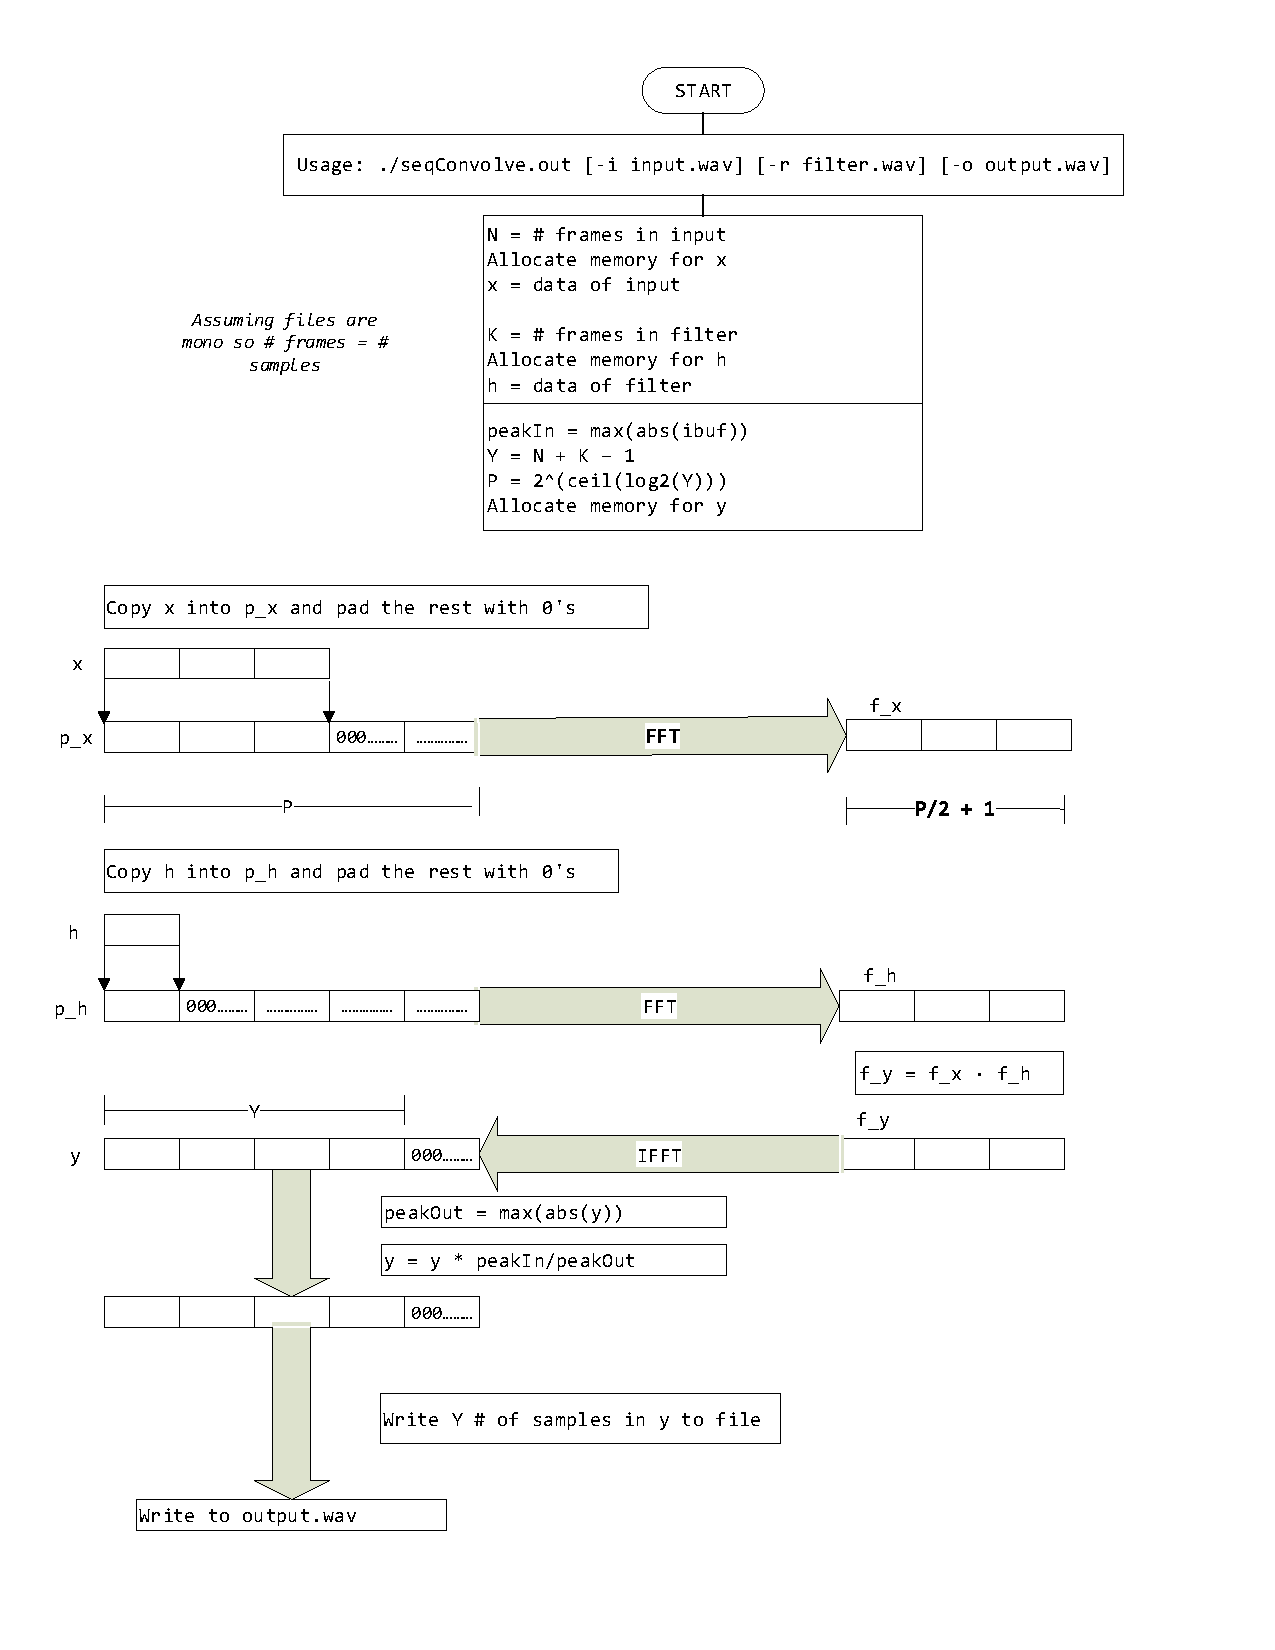
\includepdf[pages=1,pagecommand={\excerpt}]{Algorithms.pdf}
\end{changemargin}

\begin{minted}{cpp}
Frequency Domain Convolution Algorithm

read input.wav into x
read filter.wav into h
N = length of x
K = length of h

/*Find peak of input*/
peakIn = 0
for i in x:
    if | i | > peakIn:
        peakIn = i

/*Find length of output and padded length*/
Y = N + K - 1
P = pow(2, ceil(log2(Y)))

/*Copy x and h into p_x and p_h*/
p_x[0 : N - 1] = x
p_h[0 : K - 1] = h

/*Pad p_x and p_h with zeros*/
p_h[K : P - 1] = 0
p_x[N : P - 1] = 0

/*Take the Fourier transform*/
f_x = fft(x)
f_h = fft(h)

/*Convolution*/
f_y = f_x * f_h

/*Take the inverse Fourier transform*/
y = ifft(f_y)
        
/*Find peak of output*/
peakOut = 0
for i in y:
    if | i | > peakOut:
        peakOut = i
        
/*Scale all points in output*/
for n in y:
    n = n * peakIn / peakOut

/*(Optional) Write to output file*/
write y[0 : Y - 1] to output.wav
\end{minted}

\paragraph{Complex Multiplication} \hspace{0pt} \\
\indent An important point to note is that pointwise multiplication of the transformed signals is complex multiplication. C recognizes the complex number as a structure of two floats, so there needs to be a separate multiply function. 

$$(a_1 + b_1j) \cdot (a_2 + b_2j) = $$
$$a_1a_2 + a_1b_2j + a_2b_1j - b_1b_2 =$$
$$ a_1a_2 - b_1b_2 + a_1b_2j + a_2b_1j$$

The FFTW library incorporates a complex structure called \verb|fftwf_complex|. This is compatible with the complex numbers defined in C99's \verb|#include <complex.h>|. The real part and imaginary parts are stored as if the number were a two element array, with the real part coming first.
\begin{minted}{cpp}
void pointwiseMultiplication(fftwf_complex *f_x, fftwf_complex *f_h,  long long paddedFrames){
    ...
   
    for(long long i = 0; i < paddedFrames / 2 + 1; i++){
        fftwf_complex temp;
        temp[0] = f_x[i][0];
        temp[1] = f_x[i][1];
        f_x[i][0] = temp[0] * f_h[i][0] - temp[1] * f_h[i][1];
        f_x[i][1] = temp[0] * f_h[i][1] + temp[1] * f_h[i][0];
    }
    ...
}
\end{minted}

\paragraph{Overlap-Add Block Convolution} \hspace{0pt} \\
\indent Overlap-add is a divide and conquer algorithm for convolution, exploiting the fact that the convolution operation is a linear system. It's a divide and conquer algorithm in how a large input is divided into several chunks. These chunks don't necessarily need to be the same size, but they often are for programming ease. These chunks are convolved individually. Then, to fit the pieces back together, $K-1$ samples of the beginning and end of each block are pointwise added to the end and beginning (respectively) of the following and previous block. 

I utilized the algorithm while doing frequency domain convolution in case I couldn't allocate enough memory for the program. This happened when my input was $2^{30}$ samples. For an input of $2^{30}$ samples and a filter of $480,000$ samples, I would need to allocate two buffers $2^{31}$ samples or $2^{33}$ bytes long. For the complex part, I would've need to allocate two buffers $2^{30} + 1$ samples or $8 \cdot (2^{30} + 1)$ bytes. \verb|malloc()| failed for that sheer number of contiguous bytes in memory. For the sequential code, I used recursion to implement the overlap-add algorithm. My full source code for the example can be found in the appendix. 

\begin{changemargin}
\def\excerpt{\thispagestyle{empty} \paragraph{Overlap-Add Block Algorithm} \hspace{0pt} \\}
\includepdf[pages=2,pagecommand={\excerpt}]{Algorithms.pdf}
\end{changemargin}